The algorithm can only accept structured data, meaning that the input needs to have a static \emph{schema}.
The schema defines the name and position of the columns in the data table.
Recall from Chapter~\ref{subsec:cost_graph_construction}, that in order to calculate the cost graph, the algorithm needs to summarize the \textit{scaled generalization cost} for each dimension.
This implies, that for each column we also need to provide the corresponding \emph{generalizer}.
Note, that as part of the input validation, the generalizer is also validated.

Once the schema is established, we can fill up the data table by providing the row data.
Finally, by providing the \textit{k} anonymity parameter, the input is fully defined.

\begin{figure}[ht]
    \centering


    \tikzset{every picture/.style={line width=0.75pt}} %set default line width to 0.75pt

    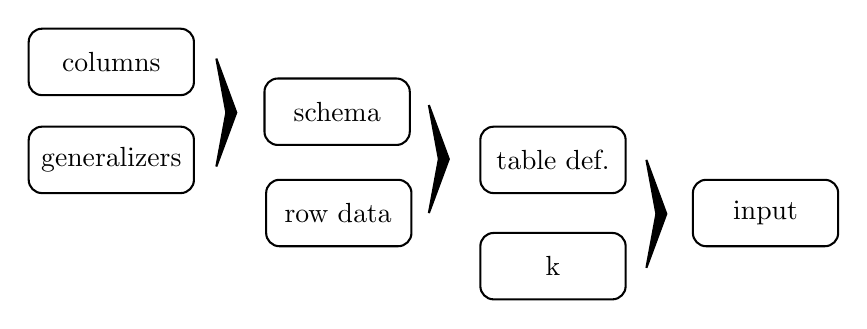
\begin{tikzpicture}[x=0.75pt,y=0.75pt,yscale=-0.8,xscale=0.8]
        %uncomment if require: \path (0,262); %set diagram left start at 0, and has height of 262

        %Rounded Rect [id:dp2859506469156541]
        \draw   (164,56) .. controls (164,51.58) and (167.58,48) .. (172,48) -- (243.5,48) .. controls (247.92,48) and (251.5,51.58) .. (251.5,56) -- (251.5,80) .. controls (251.5,84.42) and (247.92,88) .. (243.5,88) -- (172,88) .. controls (167.58,88) and (164,84.42) .. (164,80) -- cycle ;

        %Rounded Rect [id:dp5765918038864581]
        \draw   (165,117) .. controls (165,112.58) and (168.58,109) .. (173,109) -- (244.5,109) .. controls (248.92,109) and (252.5,112.58) .. (252.5,117) -- (252.5,141) .. controls (252.5,145.42) and (248.92,149) .. (244.5,149) -- (173,149) .. controls (168.58,149) and (165,145.42) .. (165,141) -- cycle ;

        %Rounded Rect [id:dp31934635079152884]
        \draw   (294,85) .. controls (294,80.58) and (297.58,77) .. (302,77) -- (373.5,77) .. controls (377.92,77) and (381.5,80.58) .. (381.5,85) -- (381.5,109) .. controls (381.5,113.42) and (377.92,117) .. (373.5,117) -- (302,117) .. controls (297.58,117) and (294,113.42) .. (294,109) -- cycle ;

        %Rounded Rect [id:dp19290025787293064]
        \draw   (22,26) .. controls (22,21.58) and (25.58,18) .. (30,18) -- (113.5,18) .. controls (117.92,18) and (121.5,21.58) .. (121.5,26) -- (121.5,50) .. controls (121.5,54.42) and (117.92,58) .. (113.5,58) -- (30,58) .. controls (25.58,58) and (22,54.42) .. (22,50) -- cycle ;
        %Rounded Rect [id:dp15065747396459095]
        \draw   (22,85) .. controls (22,80.58) and (25.58,77) .. (30,77) -- (113.5,77) .. controls (117.92,77) and (121.5,80.58) .. (121.5,85) -- (121.5,109) .. controls (121.5,113.42) and (117.92,117) .. (113.5,117) -- (30,117) .. controls (25.58,117) and (22,113.42) .. (22,109) -- cycle ;
        \draw  [fill={rgb, 255:red, 0; green, 0; blue, 0 }  ,fill opacity=1 ] (135,36) -- (147,68.5) -- (135,101) -- (141,68.5) -- cycle ;
        \draw  [fill={rgb, 255:red, 0; green, 0; blue, 0 }  ,fill opacity=1 ] (263,64) -- (275,96.5) -- (263,129) -- (269,96.5) -- cycle ;
        %Rounded Rect [id:dp5144795126994468]
        \draw   (294,149) .. controls (294,144.58) and (297.58,141) .. (302,141) -- (373.5,141) .. controls (377.92,141) and (381.5,144.58) .. (381.5,149) -- (381.5,173) .. controls (381.5,177.42) and (377.92,181) .. (373.5,181) -- (302,181) .. controls (297.58,181) and (294,177.42) .. (294,173) -- cycle ;

        \draw  [fill={rgb, 255:red, 0; green, 0; blue, 0 }  ,fill opacity=1 ] (394,97) -- (406,129.5) -- (394,162) -- (400,129.5) -- cycle ;
        %Rounded Rect [id:dp6969860888238992]
        \draw   (422,117) .. controls (422,112.58) and (425.58,109) .. (430,109) -- (501.5,109) .. controls (505.92,109) and (509.5,112.58) .. (509.5,117) -- (509.5,141) .. controls (509.5,145.42) and (505.92,149) .. (501.5,149) -- (430,149) .. controls (425.58,149) and (422,145.42) .. (422,141) -- cycle ;


        % Text Node
        \draw (337.75,97) node  [align=left] {table def.};
        % Text Node
        \draw (207.75,68) node  [align=left] {schema};
        % Text Node
        \draw (208.25,129) node  [align=left] {row data};
        % Text Node
        \draw (71.75,97) node [scale=1] [align=left] {generalizers};
        % Text Node
        \draw (71.75,38) node [scale=1] [align=left] {columns};
        % Text Node
        \draw (337.75,161) node  [align=left] {k};
        % Text Node
        \draw (465.75,129) node  [align=left] {input};


    \end{tikzpicture}
\end{figure}

\subsubsection{Example input declaration}

Listing~\ref{lst:example_input_table} shows an example usage of how to declare an input table for the anonymizer algorithm.
For simplicity's sake we assume, that a \texttt{g} map exists, which contains an appropriate generalizer for each column we use in the schema. (We will discuss how exactly generalizers are built in Section~\ref{sec:generalization}).

\begin{lstlisting}[caption=Input data table declaration,label=lst:example_input_table,float,floatplacement=H]
// g map contains a generalizer for each column
var g map[string]generalization.Generalizer
t := NewTable(&Schema{
Columns: []*Column{
    NewColumn("Name",    g["Name"]),
    NewColumn("Age",     g["Age"]),
    NewColumn("Salary",  g["Salary"]),
    NewColumn("Disease", g["Disease"]),
    },
})
t.AddRow("Joe", 30, 60000, "Flu")
t.AddRow("Eve", 27, 58000, "Sore throat")
\end{lstlisting}